\section{Introduction}

Several branches of Earth Sciences have demonstrated the importance of the
``spatiality" of the data on a microscopic scale, mainly in geochemistry and
geochronology applications where it is possible to perform punctual analysis
and compositional maps, allowing significant advances in the understanding of
igneous, metamorphic and sedimentary processes \citep{Verberne2020, Barnes2019,
Davidson2007}. Classical paleomagnetic techniques, on the other hand, consist
in analyzing bulk samples, where the magnetic signal of a single specimen is
the result of the sum of moments of a large assembly of ferromagnetic grains
\citep{Dunlop1997}. Typically, a standard paleomagnetic sample of
approximately \qty{10}{\cm\cubed} would contain hundreds of thousands
to millions of magnetic particles with sizes varying from magnetically stable
single-domain (SD) and vortex state grains (also called pseudo-single domain,
PSD) with sizes below \qty{1}{\um}, to large ($\gg \qty{1}{\um}$) grains with
multi-domain (MD) magnetic structures, which are less stable magnetic recorders
\citep{Berndt2016}. These large MD grains usually conceal the signal of the SD
and PSD grains, and techniques of step-wise thermal and magnetic treatments are
needed to unveil the more stable and reliable magnetic record
\citep{Tauxe2018}. Recently, magnetic microscopy techniques opened the
possibility of performing magnetic maps at the micro-scale and recovering the
magnetization of each grain, therefore enabling the separate analysis of stable
and unstable magnetic particles \citep{DeGroot2018, Lima2014, Weiss2007,
DeGroot2014}.

In order to apply magnetic microscopy to paleomagnetic studies, it is necessary
to recover from the magnetic images a large amount of individual magnetic
moments, corresponding to at least tens of thousands of stable fine-grained
grains ($< \qty{1}{\um}$), in order to provide statistical significance to the
remanence vector \citep[e.g., ][]{Berndt2016}. Nowadays, with the development of
magnetic microscopy techniques, this task is no longer limited by the
resolution of magnetic microscopes \citep{Fu2020, Weiss2007, DeGroot2018,
Glenn2017, Lima2014}, but essentially by the intrinsic problem presented by the
ambiguity in the inversion of potential field data \citep{Barbosa2011,
DeGroot2021, Oliveira2015Estimation}, and ultimately by the lack of a fast and
automated way to recover such a large number of individual magnetic moments
from a set of magnetic images \citep{CortesOrtuno2022, Lima2013, Lima2009}. A
solution to the non-uniqueness of magnetic moment inversion is to add
independent prior information, such as the position of the ferromagnetic
particles \citep{Fabian2019}. This can be obtained, for example, from X-ray
computed tomography \citep[microCT; ][]{Fabian2019, DeGroot2021, DeGroot2018}.
Nonetheless, the standard microCT techniques do not provide adequate resolution
to resolve the finer and more stable magnetic grains \citep{CortesOrtuno2022,
DeGroot2021}, whereas other more sophisticated techniques such as ptychographic
X-ray tomography \citep[e.g., ][]{Maldanis2020} are not readily available and
too time-consuming to be routinely used in paleomagnetic studies.

Another route to be explored in the inversion of magnetic microscopy images is
to obtain all the information, i.e. the magnetic moment and the position of the
sources, from the magnetic data itself \citep[e.g., ][]{Fu2020}. For that, we can
explore the techniques developed in exploration geophysics, in spite of the
differences between aeromagnetic surveys and magnetic microscopy
\citep{Lima2013}. Magnetic microscopy images commonly show the combined signal
of multiple magnetic particles and can vary greatly in wavelength, strength,
and spatial separation, depending on the NRM and location of each particle. We
usually assume that the signal measured by the magnetic microscope is the
vertical component of the magnetic induction vector ($b_z$), the measurements
are performed on a regular grid with evenly spaced grid points and at a
constant height, and the data are contaminated with random Gaussian noise and
long-wavelength noise (akin to a regional signal in aeromagnetic data). Here,
we provide a methodological routine to retrieve the individual magnetic moment
of ferromagnetic grains in magnetic microscopy images following the approach
devised by \citet{Oliveira2015Estimation} for the interpretation of
aeromagnetic anomalies. The method we propose allows one to quickly and
semi-automatically estimate the individual magnetic moment vector of the stable
magnetic carriers, making use of only the magnetic images themselves and an
assumption of approximately dipolar sources. If used on a large scale, the
method provides the means to scan large areas of the rock sample, attaining
potentially the number of magnetic moments necessary for paleomagnetic studies.


%%%%%%%%%%%%%%%%%%%%%%%%%%%%%%%%%%%%%%%%%%%%%%%%%%%%%%%%%%%%%%%%%%%%%%%%%%%%%%%
\section{Methodology}

We will achieve the goal of estimating the dipole moment of several individual
grains per image in a semi-automatic fashion by dividing the task into three
parts that can be performed independently:

\begin{enumerate}
\item \textbf{Source detection and separation:} Identify and spatially isolate
  the magnetic field caused by each source. We will do this through a
  combination of classic potential field data processing (\textit{total
  gradient amplitude}) and image processing (histogram stretching and
  equalization) and segmentation methods (watershed segmentation).
\item \textbf{Position estimation}: Estimate the 3D position of a magnetic
  particle based on the magnetic field measurements and the assumption of a
  dipolar source. This can be achieved by applying the Euler Deconvolution
  method to the data segment identified in step 1.
\item \textbf{Magnetic moment inversion:} Estimate the 3-component dipole
  moment vector by inverting the magnetic field data using the position
  obtained from Euler Deconvolution as a constraint and the assumption of a
  dipolar source. This leads to a linear inverse problem that is stable and
  computationally efficient, particularly since the inversion is performed
  separately for each data segment identified in step 1.
\end{enumerate}

In the sections below, we describe the methodology used in each step of our
proposed workflow.

\subsection{Automatic source detection and separation}

Our first task is to automatically identify the signal of individual particles
and spatially segregate the data into windows, each containing the signal of a
single particle. We implemented the following workflow to achieve this:

\begin{enumerate}
\item Calculate the \textit{total gradient amplitude} (TGA), also known as the
  3D analytic signal \citep{Roest1992Magnetic}, of the observed vertical
  component of the magnetic field. The TGA is entirely positive and tends to be
  more concentrated on top of the magnetic field sources than the observed
  magnetic field. The derivative calculation also acts as a high-pass filter,
  removing long-wavelength noise from the data.
\item Apply a contrast stretching method to re-scale the TGA to a new range
  defined by the lower and upper percentiles of the data in order to highlight
  the weaker signals, either coming from small or from deep-seated particles.
\item Use the Laplacian of Gaussian (LoG) method \citep{Kong2013} on the
  re-scaled TGA data to estimate the position and size of data windows
  containing the signal of each particle.
\end{enumerate}

The total gradient amplitude (TGA) was devised as a filter that can be applied
to aeromagnetic data to reduce the signal's dependence on the direction of
magnetization of the source and that concentrates the signal above the sources
\citep{Roest1992Magnetic, Nabighian2005}. The TGA is defined as the norm of the
gradient vector of a scalar field $f(x, y, z)$

\begin{equation}
\|\vec{\mathbf{\nabla}}f(x, y, z)\|  = \sqrt{(\partial_x f)^2 + (\partial_y f)^2 + (\partial_z f)^2}\ ,
\end{equation}

\noindent
in which $\partial_x f$ is the partial derivative of $f$ with respect to $x$
and likewise for the $y$ and $z$ directions. The partial derivatives are best
approximated using a second-order accurate central finite-difference scheme

\begin{equation}
\partial_x f(x, y, z) \approx \dfrac{f(x + \Delta x, y, z) - f(x - \Delta x, y, z)}{2 \Delta x} \ ,
\end{equation}

\noindent
and likewise for the $y$ and $z$ directions, in which $\Delta x$ is the grid
spacing (assumed to be equal in the $x$ and $y$ directions). For the $z$
component, $\Delta z = \Delta x$ and $f(x, y, z + \Delta z)$ and
$f(x, y, z - \Delta z)$ are calculated by upward and downward continuation,
respectively, performed in the wavenumber domain. The 2D maps of the $x$, $y$,
and $z$ derivatives will also be used in the Euler Deconvolution step described
below, which is known to be highly sensitive to noise in the derivatives
\citep{Saleh2012Applying}. This is why e prefer the finite-differences based
derivatives, which are less prone to amplifying short-wavelength noise than
those calculated in the wavenumber domain through the Fast Fourier Transform
(FFT).

Once we have obtained a TGA image, we apply a contrast stretching method to
re-scale the TGA values in order to highlight the weaker signals present in the
image. This is a necessary step to make sure that the blob detection algorithm
is able to identify particles causing both weak and strong signals. The
following contrast stretching operation is performed per pixel of the TGA image

\begin{equation}
\text{TGA}_{rescaled} = 2\left(\dfrac{\text{TGA} - v_{min}}{v_{max} - v_{min}}\right) - 1 \ ,
\end{equation}

\noindent
in which $v_{min}$ and $v_{max}$ are the upper and lower bounds of TGA values
that will be stretched to the range $[0, 1]$. By experimentation, we found
that values of $v_{min} = 1^\text{st}$ and $v_{max} = 99^\text{th}$
percentiles of the TGA range work well on real magnetic microscopy datasets.

The re-scaled TGA image is then used as input for a Laplacian of Gaussian (LoG)
blob detection algorithm \citep{Kong2013}. This method is able to identify the
location and size of multiple windows in the image containing ``blobs''. In our
case, the blobs are the re-scaled TGA field of each particle and the LoG method
detects the local TGA maxima. The LoG method is particularly well suited for
the detection of bright blobs on a dark background at the expense of a longer
computation time \citep{Han2016}. For the image sizes routinely found in
magnetic microscopy, the computation is fast and only needs to be performed
once per image.

\subsection{Euler Deconvolution}

Once the locations and sizes of the windows containing the isolated signals of
each particle are determined, we can apply the Euler Deconvolution (ED)
estimate of the $x$, $y$, and $z$ positions of the center of the particles
under a dipolar approximation. This technique was first proposed by
\citet{Thompson1982} under the name EULDPH and later extended to three
dimensions and renamed ``Euler Deconvolution'' by \citet{Reid1990}. ED is
traditionally performed on a set of moving windows that scan the entire
dataset, producing a large scatter of position estimates, most of which are
spurious \citep{Silva20033D}. This is only done because it is impractical to
segment an aeromagnetic dataset into individual anomalies. Fortunately,
magnetic microscopy images contain fewer elongated features (e.g., dikes and
suture zones) and regional signals (e.g., Curie depth variations) that are
difficult to separate. This makes it possible for us to produce isolated
signals for each magnetic particle through the source detection step described
above. Since each data window contains only the signal of a single particle, we
are able to apply ED and generate only a single position estimate per particle.

\begin{figure}[t]
\centering
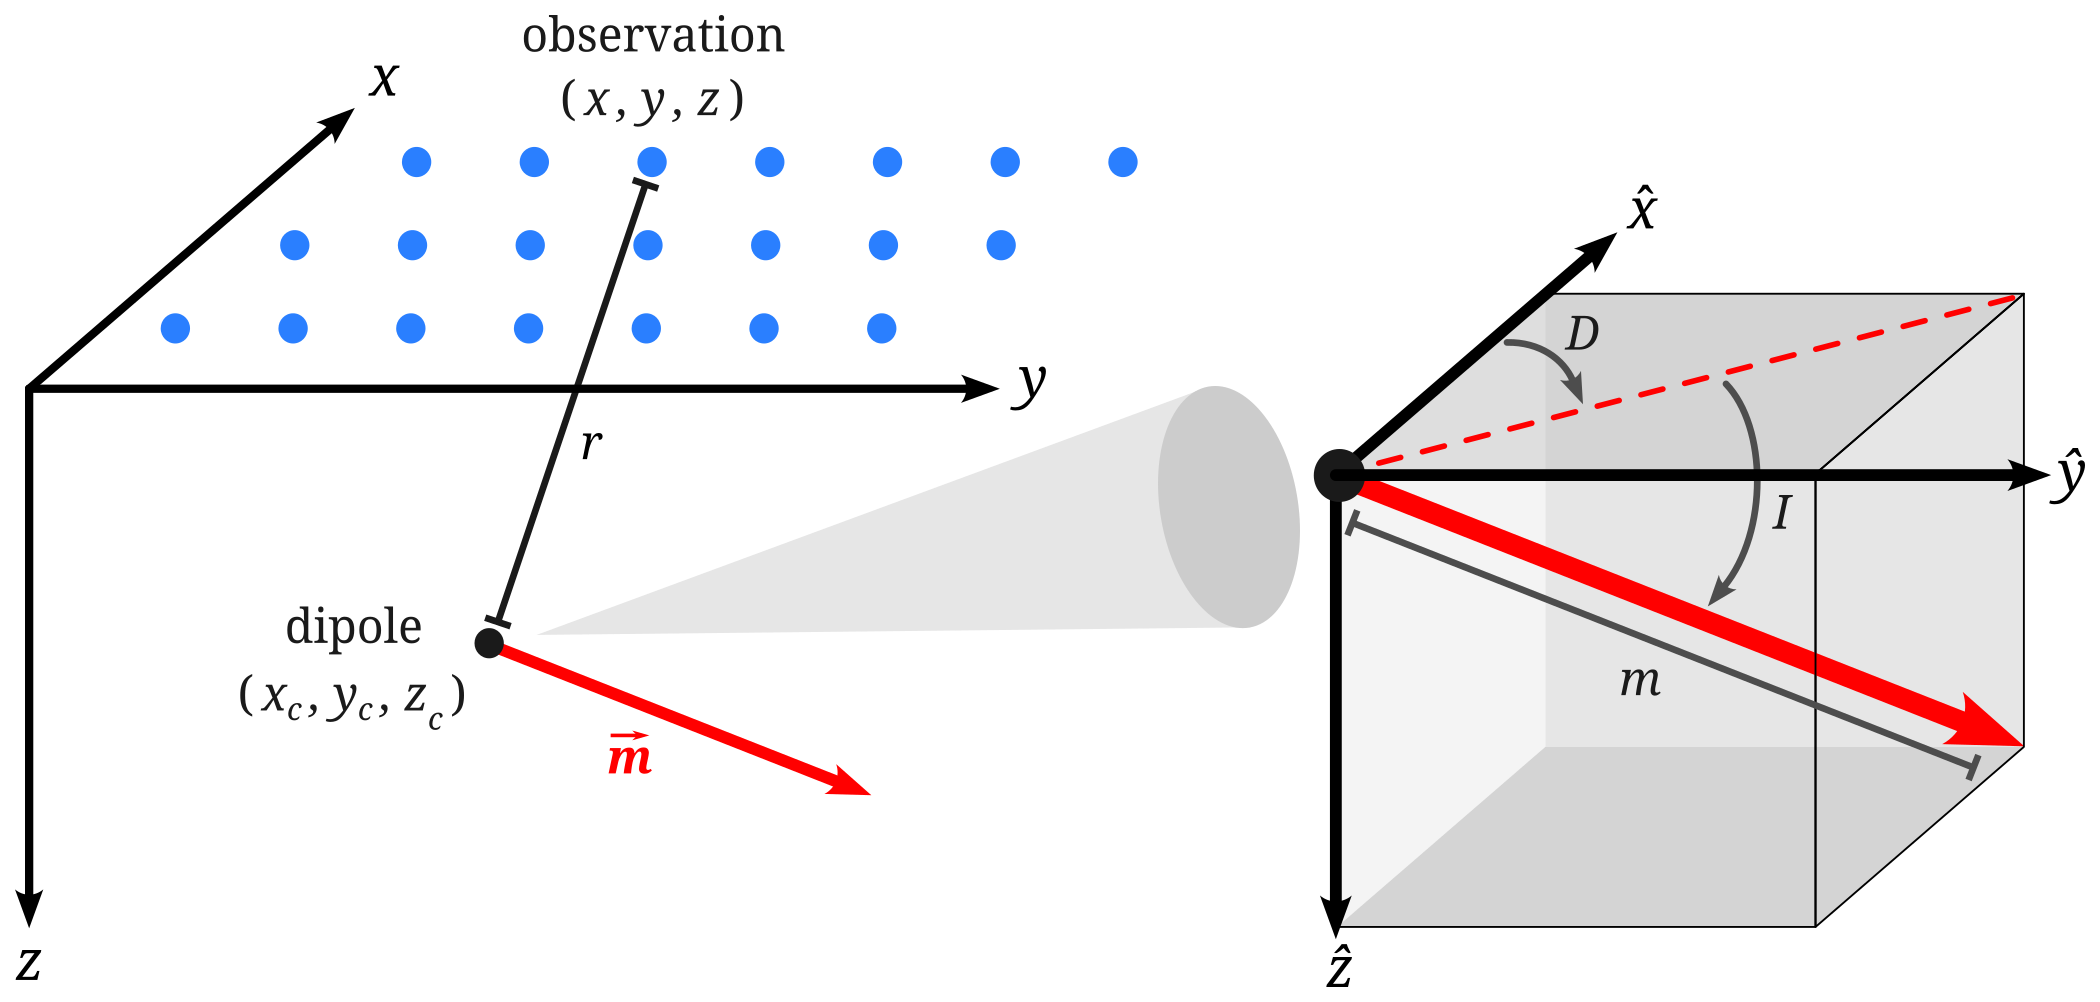
\includegraphics[width=\linewidth]{figures/coordinate-system-sketch.png}
\caption{Caption needed.}
\label{fig_coordinate_systems}
\end{figure}

Euler Deconvolution is formulated as a least-squares inversion of Euler's
homogeneity equation

\begin{equation}
\label{eq_euler_homogeneity}
(x - x_c)\partial_x f
+ (y - y_c)\partial_y f
+ (z - z_c)\partial_z f
= (b - f)\eta
\ ,
\end{equation}

\noindent
in which $(x_c, y_c, z_c)$ are the coordinates of the magnetic field source
(Figure~\ref{fig_coordinate_systems}), $b$ is the base level representing a
constant shift in the signal, and $\eta$ is the structural index corresponding
to the nature of the source \citep{Reid1990}. This equation holds true for
simple geometric sources, like spheres, dipoles, and vertical cylinders. Here,
we assume that the magnetic particles are small enough and the sensor is far
enough away that the sources can be represented by dipoles, yielding an
$\eta=3$.

The inversion is performed by rearranging Equation~\ref{eq_euler_homogeneity}
into a pseudo-parametric model with parameters $x_c$, $y_c$, $z_c$, and $b$

\begin{equation}
x_c \partial_x f + y_c \partial_x f + z_c \partial_x f + \eta b
=
x \partial_x f + y \partial_y f + z \partial_z f + \eta f
\ .
\end{equation}

Given a set of $N$ observations of the magnetic field as the harmonic function
$f$ and its spatial derivatives, we can form the $N \times 4$ system of
equations

\begin{equation}
\begin{bmatrix}
  {\partial_x f}_1 & {\partial_y f}_1 & {\partial_z f}_1 & \eta \\
  {\partial_x f}_2 & {\partial_y f}_2 & {\partial_z f}_2 & \eta \\
  \vdots & \vdots & \vdots & \vdots \\
  {\partial_x f}_N & {\partial_y f}_N & {\partial_z f}_N & \eta
\end{bmatrix}
\begin{bmatrix}
  x_c \\ y_c \\ z_c \\ b
\end{bmatrix}
=
\begin{bmatrix}
  x_1 {\partial_x f}_1 + y_1 {\partial_y f}_1 + z_1 {\partial_z f}_1 + \eta f_1 \\
  x_2 {\partial_x f}_2 + y_2 {\partial_y f}_2 + z_2 {\partial_z f}_2 + \eta f_2 \\
  \vdots \\
  x_N {\partial_x f}_N + y_N {\partial_y f}_N + z_N {\partial_z f}_N + \eta f_N \\
\end{bmatrix}
\ .
\end{equation}

In matrix notation, this linear system can be written as

\begin{equation}
\label{eq_euler_forward}
\mathbf{G} \mathbf{p} = \mathbf{h} \ .
\end{equation}

We can arrive at a solution to Equation~\ref{eq_euler_forward} by assuming that
the three spatial derivatives of $f$ have negligible error and minimizing the
misfit $\phi(\mathbf{p})$ between a pseudo-observation vector $\mathbf{h}^o$
and the predictions $\mathbf{h}$. The least-squares misfit $\phi(\mathbf{p})$
is defined as

\begin{equation}
\label{ZTSuSBbL16}
\phi(\mathbf{p}) = \|\mathbf{h}^o - \mathbf{h}\|^2 = (\mathbf{h}^o - \mathbf{G}\mathbf{p})^T (\mathbf{h}^o - \mathbf{G}\mathbf{p})\ .
\end{equation}

The minimum of $\phi(\mathbf{p})$ is obtained by solving the $4 \times 4$
system of normal equations

\begin{equation}
\mathbf{G}^T \mathbf{G} \mathbf{p} = \mathbf{G}^T \mathbf{h}^o\ .
\end{equation}

The solution vector $\hat{\mathbf{p}}$ provides an estimate of the position
$(x_c, y_c, z_c)$ and base level $b$ for the source located inside of a data
window. Repeating this process for each window produced by the source detection
algorithm will yield the horizontal locations and depths of each magnetic
particle.

\subsection{Magnetic moment inversion}

Once the source position is known and we can assume that it is approximately
spherical or dipolar, we can apply the method developed by
\citet{Oliveira2015Estimation} to estimate the dipole moment vector
$\mathbf{m}$ of the source. We begin by following
\citet{Oliveira2015Estimation} in formulating the magnetic induction vector
$\mathbf{b}$ of a dipole as

\begin{equation}
\label{eq_vector_dipole_field}
\mathbf{b}
=
\begin{bmatrix}
  b_x \\ b_y \\ b_z
\end{bmatrix}
= \dfrac{\mu_0}{4\pi}
\begin{bmatrix}
    \dfrac{\partial^2}{\partial x \partial x} \dfrac{1}{r}
  & \dfrac{\partial^2}{\partial x \partial y} \dfrac{1}{r}
  & \dfrac{\partial^2}{\partial x \partial z} \dfrac{1}{r}
  \\
    \dfrac{\partial^2}{\partial y \partial x} \dfrac{1}{r}
  & \dfrac{\partial^2}{\partial y \partial y} \dfrac{1}{r}
  & \dfrac{\partial^2}{\partial y \partial z} \dfrac{1}{r}
  \\
  \dfrac{\partial^2}{\partial z \partial x} \dfrac{1}{r}
  & \dfrac{\partial^2}{\partial z \partial y} \dfrac{1}{r}
  & \dfrac{\partial^2}{\partial z \partial z} \dfrac{1}{r}
\end{bmatrix}
\begin{bmatrix}
  m_x \\ m_y \\ m_z
\end{bmatrix}
= \dfrac{\mu_0}{4\pi} \mathbf{M}\,\mathbf{m}
\ ,
\end{equation}

\noindent
in which $r = \sqrt{(x - x_c)^2 + (y - y_c)^2 + (z - z_c)^2}$ is the Cartesian
distance between the observation point $(x, y, z)$ and the source $(x_c, y_c,
z_c)$ and $\mu_0$ is the vacuum magnetic permeability. Most magnetic
microscopes provide measurements of only the vertical component $b_z$, which
can be isolated from Equation~\ref{eq_vector_dipole_field} as

\begin{equation}
\label{eq_dipole_bz}
b_z
= \dfrac{\mu_0}{4\pi}
\begin{bmatrix}
\dfrac{\partial^2}{\partial z \partial x} \dfrac{1}{r}
& \dfrac{\partial^2}{\partial z \partial y} \dfrac{1}{r}
& \dfrac{\partial^2}{\partial z \partial z} \dfrac{1}{r}
\end{bmatrix}
\begin{bmatrix}
m_x \\ m_y \\ m_z
\end{bmatrix}
= \dfrac{\mu_0}{4\pi} \mathbf{M_z}\,\mathbf{m}
\ .
\end{equation}

The three second-order derivatives in Equation~\ref{eq_dipole_bz} are

\begin{equation}
\begin{aligned}
\dfrac{\partial^2}{\partial z \partial x} \dfrac{1}{r} &=
\dfrac{3(z - z_c)(x - x_c)}{r^5}\ ,
\\
\dfrac{\partial^2}{\partial z \partial y} \dfrac{1}{r} &=
\dfrac{3(z - z_c)(y - y_c)}{r^5}\ ,
\\
\dfrac{\partial^2}{\partial z \partial z} \dfrac{1}{r} &=
\dfrac{3(z - z_c)^2}{r^5} - \dfrac{1}{r^3}\ .
\end{aligned}
\end{equation}

Given a set of $N$ observations of $b_z$ made inside a window containing a
single source, we can form the $N \times 3$ linear equation system

\begin{equation}
\label{CgjOtKLQKT}
\begin{bmatrix}
\dfrac{\mu_0}{4\pi}\dfrac{3(z_1 - z_c)(x_1 - x_c)}{r_1^5}
& \dfrac{\mu_0}{4\pi}\dfrac{3(z_1 - z_c)(y_1 - y_c)}{r_1^5}
& \dfrac{\mu_0}{4\pi}\left(\dfrac{3(z_1 - z_c)^2}{r_1^5} - \dfrac{1}{r_1^3}\right)
\\
\dfrac{\mu_0}{4\pi}\dfrac{3(z_2 - z_c)(x_2 - x_c)}{r_2^5}
& \dfrac{\mu_0}{4\pi}\dfrac{3(z_2 - z_c)(y_2 - y_c)}{r_2^5}
& \dfrac{\mu_0}{4\pi}\left(\dfrac{3(z_2 - z_c)^2}{r_2^5} - \dfrac{1}{r_2^3}\right)
\\
\vdots & \vdots & \vdots
\\
\dfrac{\mu_0}{4\pi}\dfrac{3(z_N - z_c)(x_N - x_c)}{r_N^5}
& \dfrac{\mu_0}{4\pi}\dfrac{3(z_N - z_c)(y_N - y_c)}{r_N^5}
& \dfrac{\mu_0}{4\pi}\left(\dfrac{3(z_N - z_c)^2}{r_N^5} - \dfrac{1}{r_N^3}\right)
\end{bmatrix}
\begin{bmatrix}
m_x \\ m_y \\ m_z
\end{bmatrix}
=
\begin{bmatrix}
{b_z}_1 \\ {b_z}_2 \\ \vdots \\ {b_z}_L
\end{bmatrix}
\ ,
\end{equation}

\noindent
which can also be expressed in matrix form as

\begin{equation}
\label{qdhqM4s9Ln}
\mathbf{A} \mathbf{m} = \mathbf{d} \ .
\end{equation}

As with Euler Deconvolution, we can find a dipole moment vector that best fits
a set of $N$ observations of the vertical component of the magnetic field
$\mathbf{d}^o$ in a least-squares sense by minimizing the misfit function

\begin{equation}
\label{uV9pRVYO4l}
\Gamma (\mathbf{m}) = \| \mathbf{d}^o - \mathbf{d} \|^2 = (\mathbf{d}^o - \mathbf{A}\mathbf{m})^T  (\mathbf{d}^o - \mathbf{A}\mathbf{m})\ .
\end{equation}

\noindent
The dipole moment vector that minimizes $\Gamma (\mathbf{m})$ can be found by
solving the $3 \times 3$ normal equation system

\begin{equation}
\mathbf{A}^T \mathbf{A} \mathbf{m} = \mathbf{A}^T\mathbf{d}^o\ .
\end{equation}

\noindent
The estimated dipole moment vector $\hat{\mathbf{m}}$ can be converted into
declination $D$, inclination $I$, and magnitude $m$, which are more intuitive
quantities for interpreting paleomagnetic results, like so

\begin{equation}
  \label{eq_vector_to_incdec}
\begin{aligned}
I &= \tan^{-1}\left(\dfrac{m_z}{\sqrt{m_x^2 + m_y^2}}\right) \ , \\
D &= \tan^{-1}\left(\dfrac{m_x}{m_y}\right) \ , \\
m &= \sqrt{m_x^2 + m_y^2 + m_z^2} \ .
\end{aligned}
\end{equation}

It's important to note that these are not paleomagnetic declination and
inclination angles, but are instead related to the sample coordinate system. To
obtain the paleomagnetic direction, the dipole moment vector must be rotated to
the sample field orientation prior to the application of
Equation~\ref{eq_vector_to_incdec}.

MISSING PARAGRAPH ABOUT THE COVARIANCE ESTIMATION AND $\sigma_0$.

\begin{equation}
\label{lPOQaqlV3N}
\mathbf{C} =
\begin{bmatrix}
\sigma_x^2 & \sigma_{xy} & \sigma_{xz} \\
\sigma_{yx} & \sigma_y^2 & \sigma_{yz} \\
\sigma_{zx} & \sigma_{zy} & \sigma_z^2
\end{bmatrix}
=
\sigma_0^2 (\mathbf{A}^T\mathbf{A})^{-1}
\end{equation}

From the main diagonal of $\mathbf{C}$ we can obtain the variances of the
declination $\sigma_D^2$, inclination $\sigma_I^2$, and magnitude $\sigma_m^2$
by propagation of uncertainties

\begin{equation}
\begin{aligned}
\sigma_D^2 &= \dfrac{m_y^2\sigma_x^2 + m_x^2\sigma_y^2}{\left(m_x^2 + m_y^2\right)^2} \ , \\
\sigma_I^2 &= \dfrac{m_x^2 m_z^2 \sigma_x^2 + m_y^2 m_z^2 \sigma_y^2 + \left(m_x^2 + m_y^2\right)^2\sigma_z^2}{\left(m_x^2 + m_y^2\right) m^4} \ , \\
\sigma_m^2 &= \dfrac{m_x^2\sigma_x^2 + m_y^2\sigma_y^2 + m_z^2\sigma_z^2}{m^2} \ .
\end{aligned}
\end{equation}

\noindent
These variances reflect the sensitivity of the estimated dipole moment to
random noise in the magnetic field observations. However, they do not capture
other, often larger, sources of uncertainty like systematic errors in the
observations, data positioning errors, and the validity of the dipolar
approximation. Therefore, we recommend that these estimated variances be
treated with caution and should not be interpreted as ``the degree of certainty
that the estimated values are the true values''.

[FALAR SOBRE O CALCULO DE R2]

[INCLUIR A ESTIMATIVA DE NÃO-DIPOLARIDADE]


%%%%%%%%%%%%%%%%%%%%%%%%%%%%%%%%%%%%%%%%%%%%%%%%%%%%%%%%%%%%%%%%%%%%%%%%%%%%%%%
\section{Application to synthetic data}

We first applied our inversion workflow to synthetic data to evaluate its
strengths and limitations. The first set of synthetic data is simple and
intended to test the method's performance under ideal circumstances. The second
set is more complex, with a greater number of magnetic particles and
long-wavelength noise, and is intended to demonstrate the capabilities and
limitations of the method under real-world scenarios.

The first synthetic model was performed by generating the vertical magnetic
field derived from a simple set of four spheres with similar magnetization
intensity and radius, but completely different magnetization directions,
contaminated by high-frequency noise. This simplified test model is basically
done to investigate the efficiency of the inversions used for Euler positioning
and magnetization parameters, thus being a validation of the methodology.

The second model contains one hundred spheres with different radii and
magnetization intensities but magnetized in a similar direction within one
standard deviation. The magnetic field generated from these sources is
corrupted by both low and high-frequency noise. The complexity of this
synthetic data seeks to more faithfully emulate real magnetic microscopy data.


\subsection{Simple simulation: Validating the methodology}

\begin{figure}[tbp]
\centering
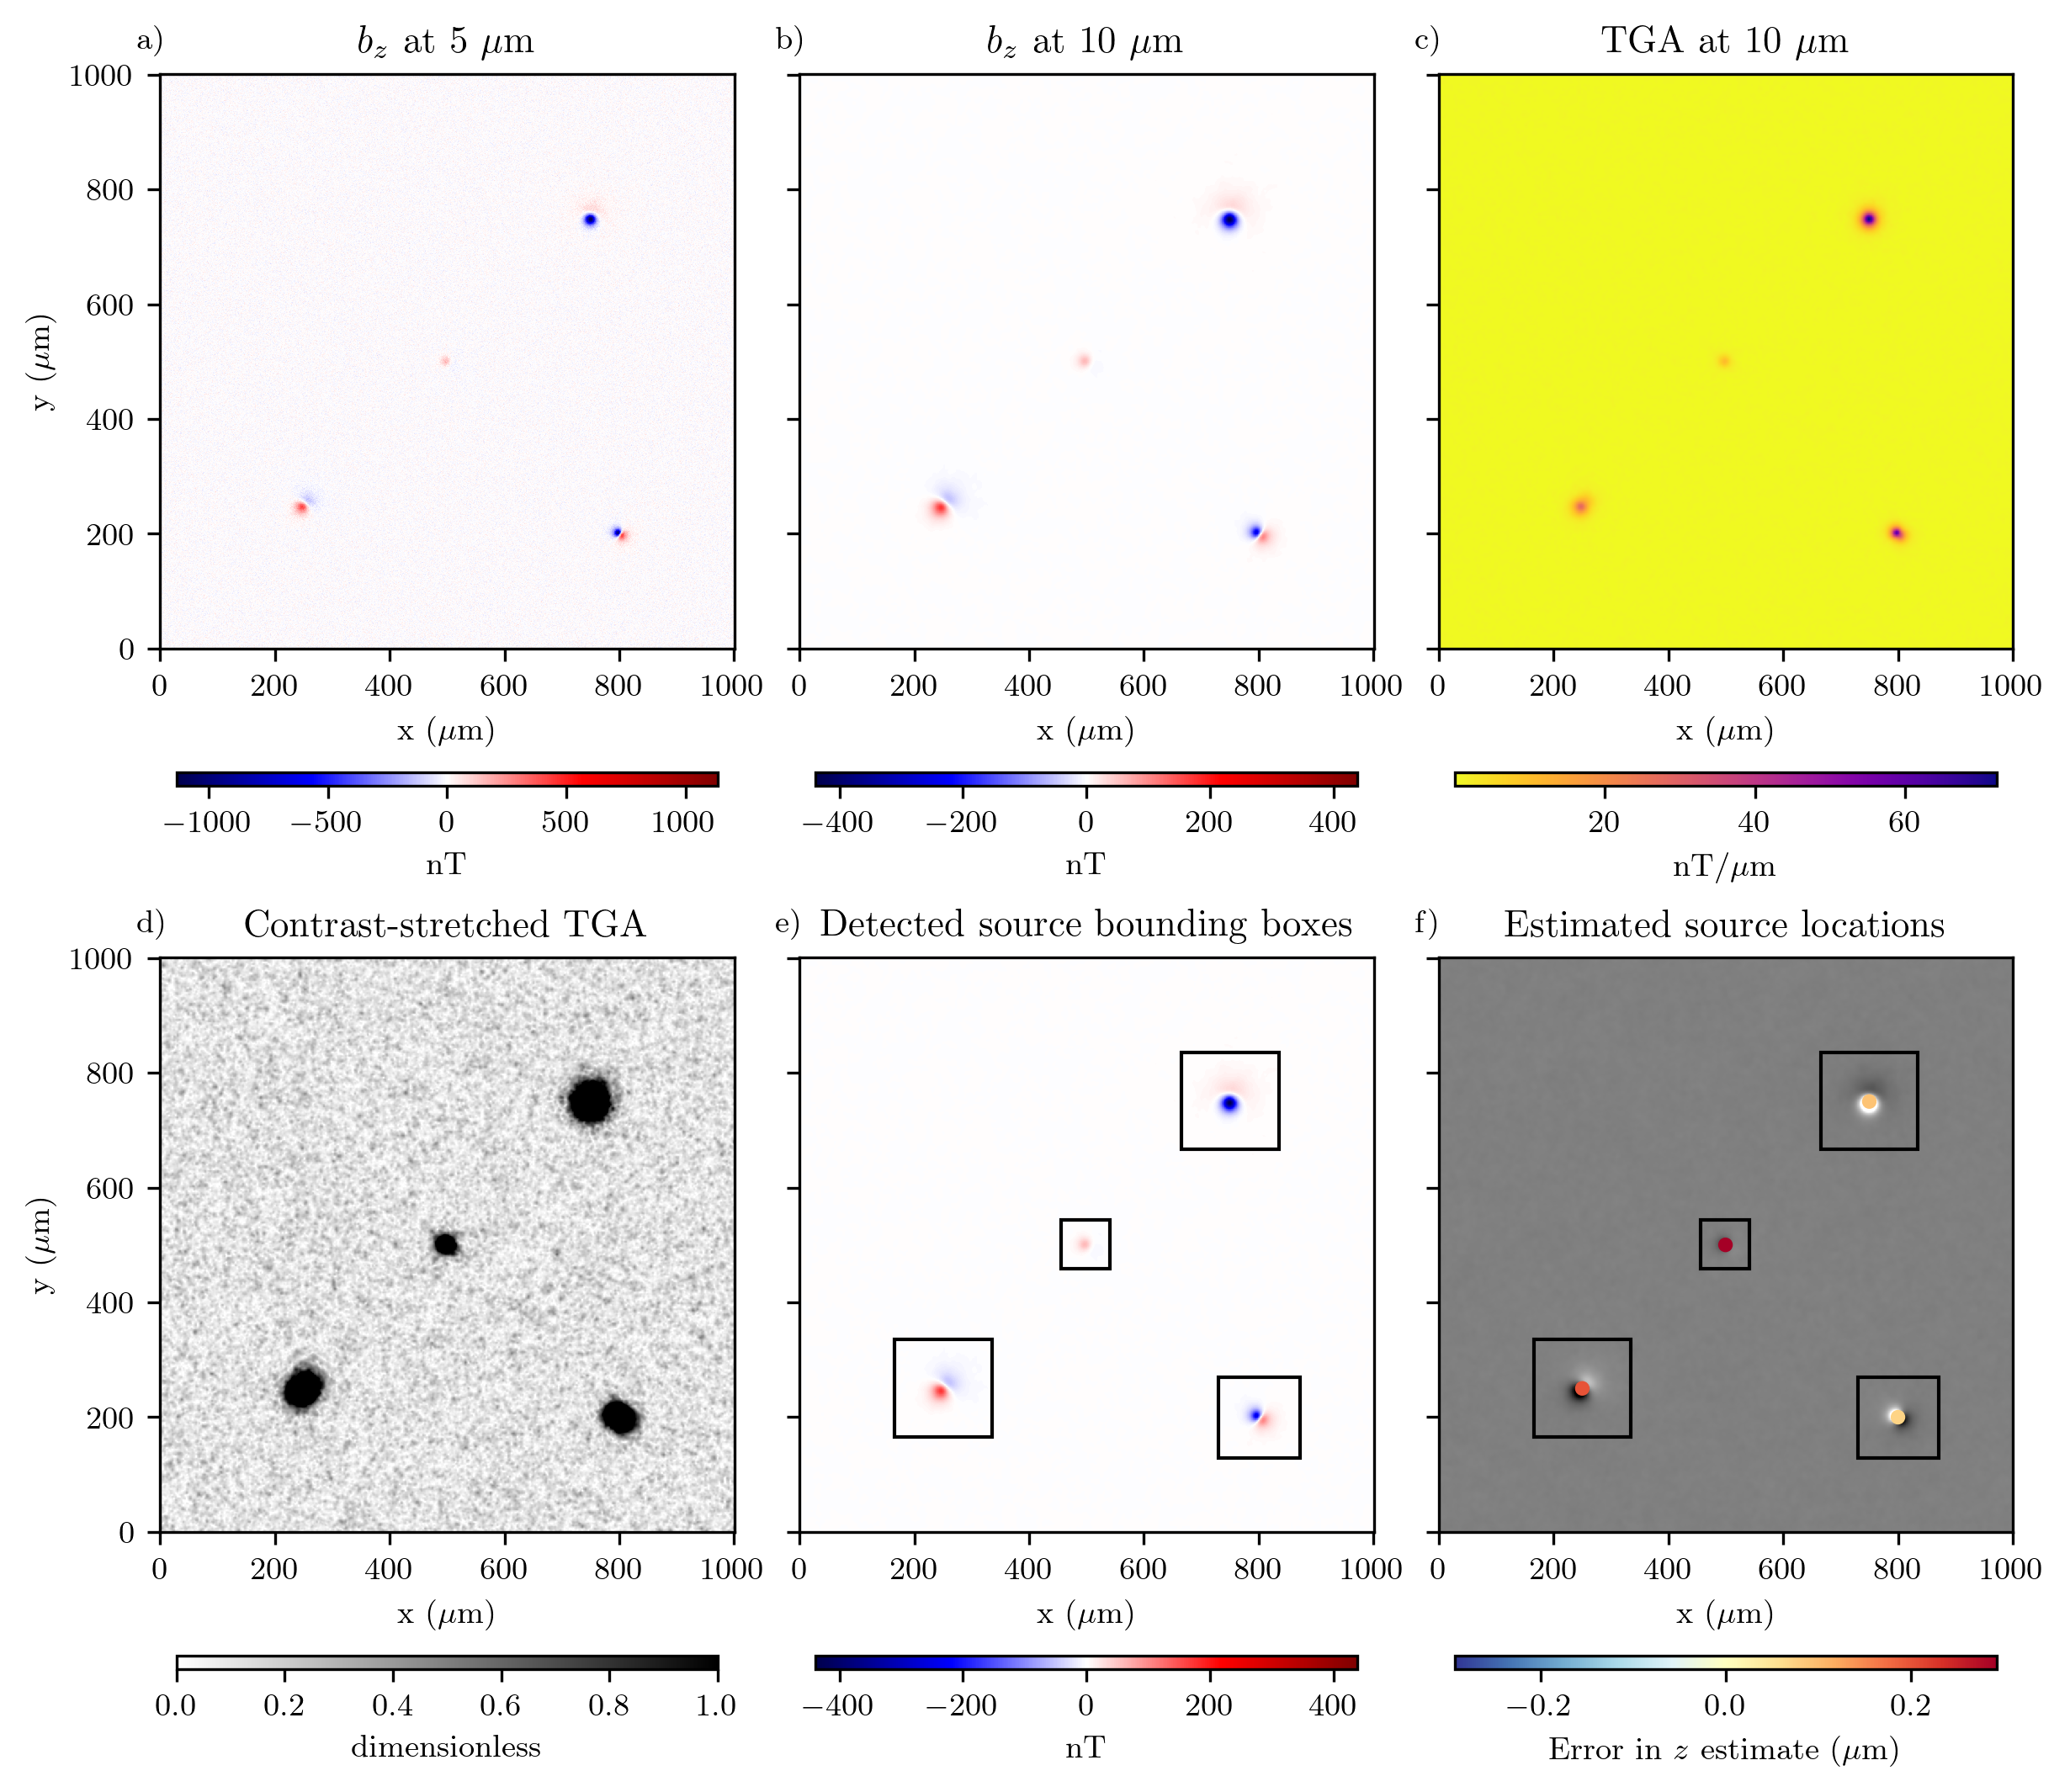
\includegraphics[width=1\linewidth]{figures/simple-synthetic-data.png}
\caption{
  a) Synthetic data contaminated with psedo-random normal noise. b) Individual sources window position (yellow squares) obtained with the blob detection algorithm applied on the total gradient map.
}
\label{fig_synthetic_simple_data}
\end{figure}

Figure~\ref{fig_synthetic_simple_data}a shows the vertical component of the magnetic field
$b_z$ over a synthetic rock section containing four uniformly magnetized
spherical sources. The map covers a surface of $\qty{1000}{\um} \times
\qty{1000}{\um}$ with
data points in a regular grid of \qty{1}{\um} ($N = 10^6$ observations)
obtained at a sensor-sample distance of \qty{5}{\um}. The magnetic field data is
contaminated with a pseudo-random noise of normal Gaussian distribution with a
zero mean and \qty{20}{\nano\tesla} standard deviation.

We first applied an upward continuation filter to smooth out high-frequency
noise \citep{Blakely1996}, since it strongly affects the first derivatives of
the potential field required by the Euler equation. Then, we calculated the
magnetic total gradient (or horizontal gradient) filter and applied the blob
detection algorithm to the total gradient map to obtain the position of the
data window for each source (Figure~\ref{fig_coordinate_systems}b). The ED was
run for each selected source by assuming the structural index of a
sphere/punctual source, therefore obtaining the Cartesian coordinates of each
source causing the magnetic potential anomaly in the observed data set (Table
1).

\begin{figure}[!t]
\centering
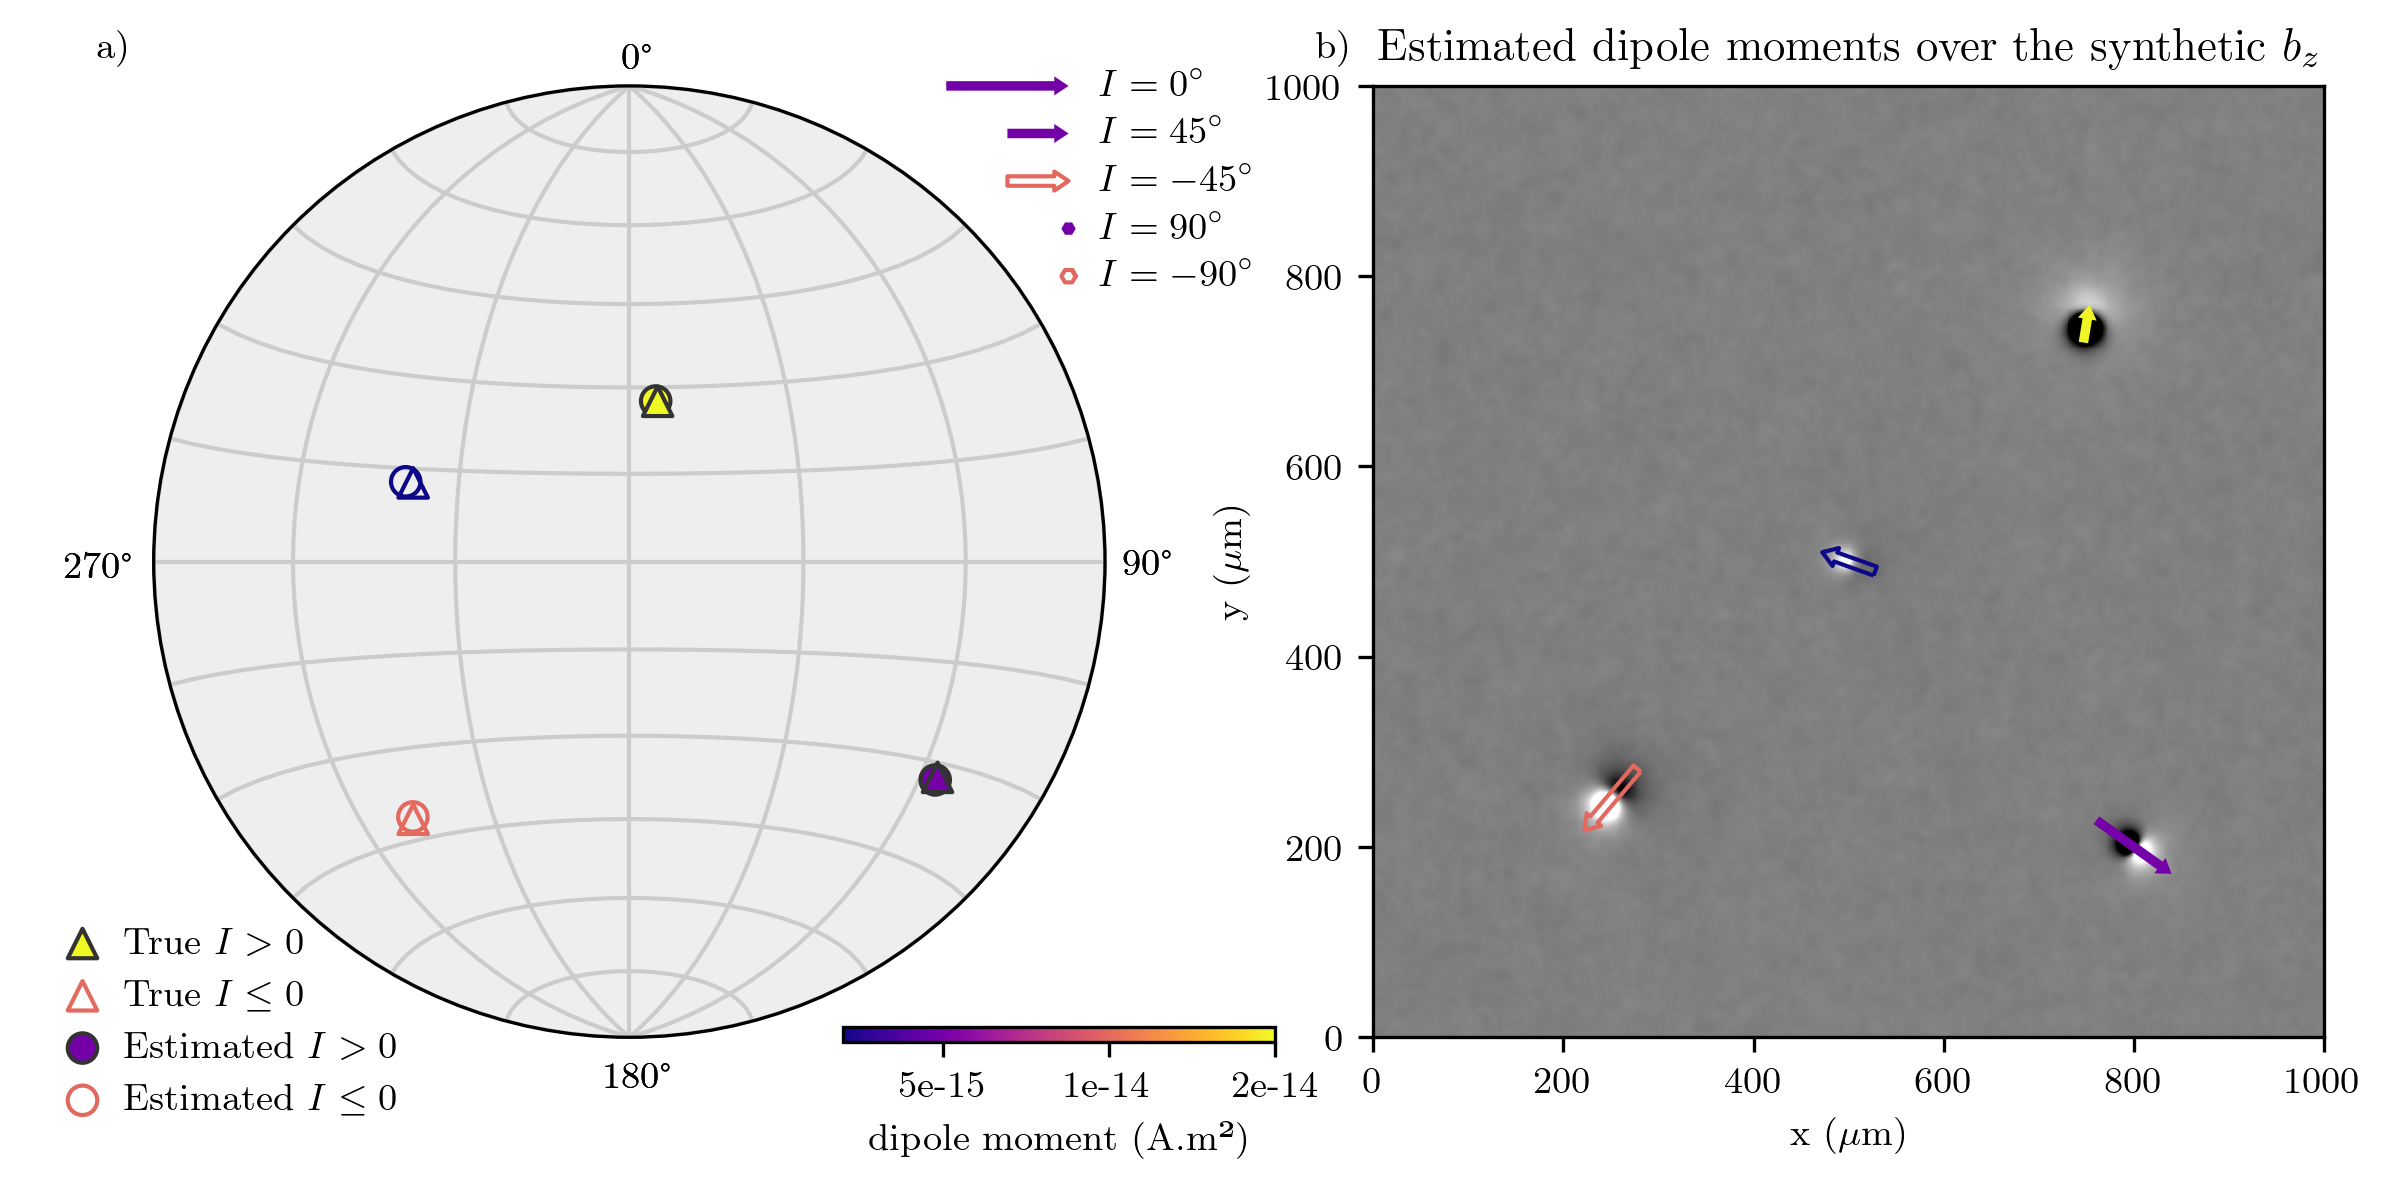
\includegraphics[width=0.75\linewidth]{figures/simple-synthetic-dipole-moment.png}
\caption{
  CAPTION NEEDED
}
\label{fig_synthetic_simple_results}
\end{figure}

The central positions of each source obtained with ED were used as an input
parameter for inverting the vertical magnetic field. The inversion produced a
least squares (or robust) approximation solution for the vector of Cartesian
magnetic moments $m_x, m_y, m_z$ and the corresponding magnetization directions
(D and I) and intensity of magnetic moment $m$. We also obtained the
uncertainty propagation of this inversion, using Equation (REFERENCE NEEDED)
and considering $\sigma = \qty{15}{\nano\tesla}$.

\begin{table}[t]
  \begin{center}
    \small
    
\begin{tabular}{ r c c c l l l } 
  \toprule
  & \multicolumn{3}{c}{Position} & \multicolumn{3}{c}{Dipole moment} \\
  & $x_c$ ($\mu$m) & $y_c$ ($\mu$m) & $z_c$ ($\mu$m) & $I$ (\textdegree) & $D$ (\textdegree) & $m$ (A.m²) \\
  \midrule
  true & 800.00 & 200.00 & -3.50 & 22.00 & 125.00 & 5.000e-15 \\
  estimated & 799.91 & 199.94 & -3.40 & 22.08 ± 0.01 & 125.52 ± 0.02 & 4.921e-15 ± 1.4e-18 \\
  true & 750.00 & 750.00 & -8.50 & 62.00 & 10.00 & 1.500e-14 \\
  estimated & 749.98 & 749.99 & -8.43 & 62.00 ± 0.01 & 9.30 ± 0.02 & 1.486e-14 ± 1.8e-18 \\
  true & 250.00 & 250.00 & -10.00 & -30.00 & -140.00 & 1.000e-14 \\
  estimated & 250.03 & 249.89 & -9.93 & -30.32 ± 0.01 & -139.70 ± 0.02 & 9.966e-15 ± 2.6e-18 \\
  true & 500.00 & 500.00 & -7.75 & -50.00 & -70.00 & 2.000e-15 \\
  estimated & 500.07 & 499.95 & -7.76 & -48.66 ± 0.05 & -70.36 ± 0.09 & 2.000e-15 ± 1.8e-18 \\
  \bottomrule
\end{tabular}

  \end{center}
  \caption{Meh}
  \label{tab_synthetic_simple_results}
\end{table}

\citet{Oliveira2015Estimation} proved that the magnetization directions (D and
I) recovered by the least squares estimator are sensitive to variations in the
horizontal coordinates of the center of the magnetic sources, but are
practically insensitive to variations in depth. Thus, they consider the Euler
deconvolution method as an adequate technique to estimate the central positions
that will be used as prior information for inversion. This occurs mainly
because, when well performed, the recovery of the horizontal coordinates of the
source central position is considerably accurate, while the vertical coordinate
can undergo greater variation even though it still provides satisfactory
results \citep{Silva20033D, Melo2013}.



%%%%%%%%%%%%%%%%%%%%%%%%%%%%%%%%%%%%%%%%%%%%%%%%%%%%%%%%%%%%%%%%%%%%%%%%%%%%%%%
\section{Acknowledgements}

We are indebted to the developers and maintainers of the open-source software
without which this work would not have been possible.
